% Provenance (never printed): BCPST year 1 geology (2021), "la carte
% geologique" (reading a map, structures, chronology), union licence
% Sciences de la Terre L1 (cartographie: strike and dip, three-point problem,
% outcrop patterns, DEM and GIS). See sources/outline_sources.md. Pilot
% chapter, 2026-10-22. The region is the series' invented Varden Hills
% (figdata/shared/region.py); every number about it is computed in
% figdata/bachelor-1/varden_maps.py or figdata/bachelor-1/v_rule.py.
\chapter{الخرائط الجيولوجية}\label{ch:b1:geological-maps}

يعبر الجيولوجي سلسلة من التلال المنخفضة حاملًا لوحة الخريطة ودفترًا وبوصلة مع مقياس الميل. ومعظم الأرض عشب أو غابة أو حقل محروث؛ ولا تظهر الصخور إلا هنا وهناك، في ضفة جدول، أو في قطع طريق، أو على حافة صخرية. ومن هذه اللمحات المتفرقة، ومن شكل الأرض، يجب على الجيولوجي أن يقول أيّ صخر يقع تحت كل متر مربع من التلال، وكيف تميل الطبقات، وأين تنكسر، وبأيّ ترتيب حدث كل ذلك. والنتيجة هي \omterm{def:b1:geological-maps:geological-map}{الخريطة الجيولوجية}: رسم مسطّح يرمّز جسمًا صخريًا ثلاثي الأبعاد. يشرح هذا الفصل كيف تُصنع مثل هذه الخريطة وكيف تُقرأ: كيف تُقاس \omterm{def:b1:geological-maps:attitude}{وضعية} سطح وتُحسب، ولماذا يرسم \omterm{def:b1:geological-maps:geological-map}{الانكشاف} لطبقة الأنماط التي يرسمها، وكيف تروي الخريطة تاريخًا. وتأتي أمثلتها من منطقة متخيَّلة لكنها متّسقة جيولوجيًا، هي تلال فاردن، التي تتكرر في هذا الكتاب.

\begin{recall}
يُظهر الخريطة الطبوغرافية التضاريس بخطوط الكنتور، أي خطوط الارتفاع المتساوي؛ ومقياس رسمها يربط المسافات على الخريطة بالمسافات على الأرض (الكتاب 1، الصف 9). وتُستنتج الأعمار النسبية من التراكب (الطبقة أحدث من الطبقات التي تحتها، ما لم يُقلب التتابع)، ومن القطع المتقاطع (ما يقطع صخرًا أحدث منه)، ومن الاحتواء (الكتاب 1، الصف 7). والصدع كسر تنزاح على طوله كتلتان (الكتاب 1، الصف 7)؛ أما هندسة \omterm{def:b1:geological-maps:fold}{الطيات} والصدوع فموضوع \cref{ch:b1:faults-folds-fabrics}.
\end{recall}

\section{الخريطة قطعٌ في ثلاثة أبعاد}\label{sec:b1:geological-maps:cut}

\begin{definition}[الخريطة الجيولوجية]\label{def:b1:geological-maps:geological-map}
تُظهر \emph{الخريطة الجيولوجية}\index{الخريطة الجيولوجية}، عند كل نقطة من سطح الأرض، الوحدة الصخرية التي تقع هناك تحت التربة، مع \emph{التماسات}\index{التماس (جيولوجي)} --- وهي الأسطح الفاصلة بين وحدتين --- والبنى (الصدوع، ومحاور \omterm{def:b1:geological-maps:fold}{الطيات}، ووضعيات الطبقات) التي تؤثّر فيها. و\emph{الوحدة الصخرية المرسومة}\index{الوحدة الصخرية} جسم من الصخر يمكن تمييزه وتتبّعه في الحقل، ويُرسم بلون واحد؛ و\emph{انكشافها}\index{الانكشاف} هو المساحة التي تقع فيها على السطح.
\end{definition}

\begin{definition}[نموذج الارتفاع الرقمي]\label{def:b1:geological-maps:dem}
\emph{نموذج الارتفاع الرقمي}\index{نموذج الارتفاع الرقمي} شبكة من الارتفاعات الأرضية، $z = g(x,y)$، عند نقاط متباعدة بانتظام. ويخزّن نظام المعلومات الجغرافية مثل هذه الشبكات، وطبقات الخريطة الأخرى (\omterm{def:b1:geological-maps:geological-map}{التماسات}، والصدوع، والقياسات، والآبار الاستكشافية) في إطار إحداثيات مشترك، ويُجري الحسابات عليها.
\end{definition}

\begin{proposition}[انكشاف التماس]\label{prop:b1:geological-maps:intersection}
لتكن الأرض السطح $z = g(x,y)$، وليكن \omterm{def:b1:geological-maps:geological-map}{التماس} السطح
$z = c(x,y)$. أثر \omterm{def:b1:geological-maps:geological-map}{التماس} على الخريطة هو المنحنى
\[
  g(x,y) = c(x,y),
\]
هو مسقط تقاطع السطحين على المستوي الأفقي. والوحدة الواقعة فوق \omterm{def:b1:geological-maps:geological-map}{التماس} تنكشف حيث يكون $g > c$.
\end{proposition}

\begin{proof}
تقع نقطة من الخريطة على الأثر إذا وفقط إذا كان سطح الأرض عند تلك النقطة ينتمي إلى \omterm{def:b1:geological-maps:geological-map}{التماس}، أي $g(x,y) = c(x,y)$. وحيث يكون $g(x,y) > c(x,y)$ تكون الأرض فوق \omterm{def:b1:geological-maps:geological-map}{التماس}: فالصخر عند السطح ينتمي إلى الوحدة التي تقع فوقه.
\end{proof}

\begin{remark}[كيف رُسمت خرائط هذا الكتاب]\label{rem:b1:geological-maps:computed}
هذا هو بالضبط ما يفعله نظام المعلومات الجغرافية حين يرسم خريطة من نموذج ثلاثي الأبعاد: فهو يحسب $g - c$ على شبكة \omterm{def:b1:geological-maps:dem}{نموذج الارتفاع الرقمي}، ويرسم المنحنيات حيث تغيّر إشارتها. وقد رُسمت خرائط تلال فاردن في هذا الكتاب بهذه الطريقة، انطلاقًا من نموذج جيولوجي تُعرف فيه كل الأسطح.
\end{remark}

\begin{omfigure}
\begin{tikzpicture}
\begin{axis}[axis equal image, xmin=0, xmax=10, ymin=0, ymax=8, width=0.82\linewidth,
  tick label style={font=\scriptsize}, xlabel={\foreignlanguage{arabic}{الشرق \babelsublr{(\unit{km})}}}, ylabel={\foreignlanguage{arabic}{الشمال \babelsublr{(\unit{km})}}},
  label style={font=\small}, colormap/blackwhite, enlargelimits=false]
\addplot[matrix plot*, mesh/cols=101, point meta=explicit, shader=interp] table[x=x_km, y=y_km, meta=shade] {figdata/out/bachelor-1-varden_maps-shade.dat};
\addplot[contour, line width=0.25pt, opacity=0.7] table {figdata/out/shared-region-contours.dat};
\addplot[index contour, opacity=0.8] table {figdata/out/shared-region-index-contours.dat};
\addplot[river] table {figdata/out/shared-region-river.dat};
\end{axis}
\end{tikzpicture}

{\small تلال فاردن كنموذج ارتفاع رقمي: الأرض مضاءة من الشمال الغربي، مع خطوط كنتور كل \qty{50}{m} (أسمك عند 250 و\qty{500}{m})، والنهر الذي يجري نحو الشرق.}
\end{omfigure}

\begin{omfigure}
\begin{tikzpicture}
\begin{axis}[axis equal image, xmin=0, xmax=10, ymin=0, ymax=8, width=0.82\linewidth,
  tick label style={font=\scriptsize}, xlabel={\foreignlanguage{arabic}{الشرق \babelsublr{(\unit{km})}}}, ylabel={\foreignlanguage{arabic}{الشمال \babelsublr{(\unit{km})}}},
  label style={font=\small}]
\addplot[lith schist, draw=black, line width=0.3pt, even odd rule] table {figdata/out/shared-region-unit-schist.dat};
\addplot[lith granite, draw=black, line width=0.3pt, even odd rule] table {figdata/out/shared-region-unit-granite.dat};
\addplot[om lith={icsTriassic!35}{om sand}, draw=black, line width=0.3pt, even odd rule] table {figdata/out/shared-region-unit-sandstone.dat};
\addplot[om lith={icsJurassic!40}{om limestone}, draw=black, line width=0.3pt, even odd rule] table {figdata/out/shared-region-unit-limestone.dat};
\addplot[om lith={icsJurassic!15}{om shale}, draw=black, line width=0.3pt, even odd rule] table {figdata/out/shared-region-unit-shale.dat};
\addplot[om lith={icsCretaceous!35}{om limestone}, draw=black, line width=0.3pt, even odd rule] table {figdata/out/shared-region-unit-chalk.dat};
% the fault is drawn before the alluvium: the younger alluvial floor conceals it
\addplot[normal fault] table {figdata/out/shared-region-fault.dat};
\addplot[lith alluvium, draw=black, line width=0.3pt, even odd rule] table {figdata/out/shared-region-unit-alluvium.dat};
\addplot[contour, opacity=0.55] table {figdata/out/shared-region-contours.dat};
\addplot[river] table {figdata/out/shared-region-river.dat};
\pic at (axis cs:4.3,6.6) {strikedip={350.6}{12}};
\pic at (axis cs:2.2,6.6) {strikedip={189.3}{12}};
\pic at (axis cs:8.6,1.4) {northarrow};
\fill[black] (axis cs:6.6,0.35) rectangle (axis cs:7.1,0.5);
\fill[white] (axis cs:7.1,0.35) rectangle (axis cs:7.6,0.5);
\fill[black] (axis cs:7.6,0.35) rectangle (axis cs:8.1,0.5);
\fill[white] (axis cs:8.1,0.35) rectangle (axis cs:8.6,0.5);
\draw[black, line width=0.4pt] (axis cs:6.6,0.35) rectangle (axis cs:8.6,0.5);
\node[font=\footnotesize, above, inner sep=1.5pt, fill=white, fill opacity=0.8, text opacity=1] at (axis cs:7.6,0.5) {\qty{2}{km}};
\end{axis}
\end{tikzpicture}

\smallskip
\begin{tikzpicture}[font=\footnotesize]
\matrix[column sep=7pt, row sep=3pt, matrix of nodes, nodes={anchor=west}] {
  \tikz\draw[black!60, line width=0.4pt, lith alluvium] (0,0) rectangle (0.7,0.32); & الطمي (الرباعي) &
  \tikz\draw[black!60, line width=0.4pt, om lith={icsCretaceous!35}{om limestone}] (0,0) rectangle (0.7,0.32); & الطباشير (\babelsublr{90 Ma}) \\
  \tikz\draw[black!60, line width=0.4pt, om lith={icsJurassic!15}{om shale}] (0,0) rectangle (0.7,0.32); & الصخر الطيني (الجوراسي، \babelsublr{165 Ma}) &
  \tikz\draw[black!60, line width=0.4pt, om lith={icsJurassic!40}{om limestone}] (0,0) rectangle (0.7,0.32); & الحجر الجيري (الجوراسي، \babelsublr{180 Ma}) \\
  \tikz\draw[black!60, line width=0.4pt, om lith={icsTriassic!35}{om sand}] (0,0) rectangle (0.7,0.32); & الحجر الرملي (الترياسي، \babelsublr{245 Ma}) &
  \tikz\draw[black!60, line width=0.4pt, lith granite] (0,0) rectangle (0.7,0.32); & الغرانيت (\babelsublr{310 Ma}) \\
  \tikz\draw[black!60, line width=0.4pt, lith schist] (0,0) rectangle (0.7,0.32); & الشيست (\babelsublr{480 Ma}) &
  \tikz\draw[normal fault] (0,0.16) -- (0.9,0.16); & الصدع العادي: الشرطات على الجانب الهابط \\
};
\end{tikzpicture}

{\small \omterm{def:b1:geological-maps:geological-map}{الخريطة الجيولوجية} لتلال فاردن، مع الكنتورات والنهر، وقياسين \omterm{def:b1:geological-maps:attitude}{للوضعية} (خط \omterm{def:b1:geological-maps:attitude}{الامتداد} وشرطة \omterm{def:b1:geological-maps:attitude}{الانحدار}، مع \omterm{def:b1:geological-maps:attitude}{الانحدار} بالدرجات)، والمفتاح. الأعمار هي أعمار وحدات المنطقة؛ والصدع مخفيّ تحت الطمي الأحدث لقاع الوادي.}
\end{omfigure}

\section{وضعية المستوي}

\begin{definition}[الامتداد، والانحدار، واتجاه الانحدار]\label{def:b1:geological-maps:attitude}
لتكن سطحًا جيولوجيًا --- سطح طبقة، أو تماسًا، أو صدعًا --- مستويًا محليًا. و\emph{الامتداد}\index{الامتداد} هو اتجاه الخطوط الأفقية التي يحويها، ويُعطى بوصفه سمتًا (بالدرجات مع عقارب الساعة من الشمال). و\emph{الانحدار}\index{الانحدار} $\delta$ هو الزاوية بين المستوي والأفق، مقيسةً في المستوي الشاقولي العمودي على الامتداد، $0 \le \delta \le \ang{90}$. و\emph{اتجاه الانحدار}\index{اتجاه الانحدار} $\alpha$ هو سمت أشدّ خط هابط في المستوي انحدارًا. وهذان معًا يكوّنان \emph{وضعية}\index{وضعية المستوي} المستوي، وتُكتب اتجاه الانحدار/الانحدار، مثل $080/12$.
\end{definition}

\begin{notation}[الامتداد وفق قاعدة اليد اليمنى]\label{not:b1:geological-maps:rhr}
يمكن قراءة \omterm{def:b1:geological-maps:attitude}{الامتداد} في اتجاهين متعاكسين. وتختار \emph{قاعدة اليد اليمنى} الاتجاه الذي يميل فيه المستوي نحو يمين الراصد الناظر على طول \omterm{def:b1:geological-maps:attitude}{الامتداد}: \omterm{def:b1:geological-maps:attitude}{الامتداد} $= \alpha - \ang{90}$ (بتردّد \ang{360}). وعلى الخريطة يكون الرمز خط امتداد عليه شرطة قصيرة تشير إلى أسفل \omterm{def:b1:geological-maps:attitude}{الانحدار}، مكتوبًا عليه \omterm{def:b1:geological-maps:attitude}{الانحدار}.
\end{notation}

\begin{omfigure}
\tdplotsetmaincoords{65}{125}
\begin{tikzpicture}[tdplot_main_coords, font=\small, scale=1.05]
  % the horizontal plane
  \fill[omSea!50] (-2.2,-1.6,0) -- (2.2,-1.6,0) -- (2.2,1.6,0) -- (-2.2,1.6,0) -- cycle;
  \draw[black!40] (-2.2,-1.6,0) -- (2.2,-1.6,0) -- (2.2,1.6,0) -- (-2.2,1.6,0) -- cycle;
  % the dipping plane: strike along y (north), dipping east (+x) at 30 degrees
  \fill[omLithLime!80, opacity=0.85] (-0.0,-1.6,0) -- (-0.0,1.6,0) -- (2.2,1.6,-1.27) -- (2.2,-1.6,-1.27) -- cycle;
  \draw[black!60] (0,-1.6,0) -- (0,1.6,0) -- (2.2,1.6,-1.27) -- (2.2,-1.6,-1.27) -- cycle;
  % strike line (horizontal, in both planes)
  \draw[omThm, line width=1.1pt] (0,-1.6,0) -- (0,1.6,0);
  % dip line and the horizontal below it, with the dip angle
  \draw[omDef, line width=1.1pt, -{Stealth[length=2.4mm]}] (0,0,0) -- (2.2,0,-1.27);
  \draw[black!60, densely dashed] (0,0,0) -- (2.2,0,0);
  \draw[black!60, densely dashed] (2.2,0,0) -- (2.2,0,-1.27);
  \draw[black] plot[domain=0:30, samples=16, variable=\t] ({0.8*cos(\t)}, 0, {-0.8*sin(\t)});
  \node[font=\footnotesize] at (1.05,0,-0.22) {$\delta$};
  % north arrow on the horizontal plane
  \draw[black, -{Stealth[length=2mm]}] (-1.8,-1.2,0) -- (-1.8,-0.3,0);
  \node[font=\footnotesize] at (-1.8,-0.05,0) {ش};
\end{tikzpicture}
\begin{tikzpicture}[font=\small]
  \node[align=left, anchor=west, text width=5.2cm] at (0,0) {%
    \textcolor{omThm}{\rule[0.5ex]{0.6cm}{1.1pt}} الامتداد: خط أفقي من المستوي؛\\[3pt]
    \textcolor{omDef}{\rule[0.5ex]{0.6cm}{1.1pt}} أشدّ خط انحدارًا في المستوي، وسمته هو اتجاه الانحدار؛\\[3pt]
    الانحدار هو الزاوية بين هذا الخط والأفق المتقطّع.};
\end{tikzpicture}

{\small مستوٍ يمتد شمالًا وينحدر \ang{30} نحو الشرق (\omterm{def:b1:geological-maps:attitude}{الوضعية} $090/30$)، ويقطع مستويًا أفقيًا على طول خط امتداده. غير مرسوم بمقياس.}
\end{omfigure}

\begin{proposition}[معادلة المستوي المائل]\label{prop:b1:geological-maps:plane}
مع $x$ نحو الشرق، و$y$ نحو الشمال، و$z$ نحو الأعلى، يكون المستوي الذي اتجاه انحداره $\alpha$ وانحداره $\delta$ ويمرّ بالنقطة $(x_0, y_0, z_0)$ هو
\[
  z = z_0 - \tan\delta\,\bigl[(x - x_0)\sin\alpha + (y - y_0)\cos\alpha\bigr].
\]
\end{proposition}

\begin{proof}
المتجهة الأفقية ذات الطول الواحد التي تشير في \omterm{def:b1:geological-maps:attitude}{اتجاه الانحدار} هي
$\vec u = (\sin\alpha, \cos\alpha, 0)$ (يُقاس \omterm{def:b1:spherical-astronomy:horizontal}{السمت} من الشمال، أي المحور $y$، نحو الشرق، أي المحور $x$). على امتداد الخط، العمودي على
$\vec u$، يكون المستوي أفقيًا؛ وعلى طول $\vec u$ ينخفض بمقدار
$\tan\delta$ لكل وحدة مسافة أفقية. والمسافة الأفقية لنقطة عن خط \omterm{def:b1:geological-maps:attitude}{الامتداد} المارّ بالنقطة $(x_0, y_0)$، مأخوذة موجبة نحو أسفل \omterm{def:b1:geological-maps:attitude}{الانحدار}، هي
$(x-x_0)\sin\alpha + (y-y_0)\cos\alpha$، ومنها تُستنتج الصيغة.
\end{proof}

\begin{theorem}[الوضعية انطلاقًا من ثلاث نقاط]\label{thm:b1:geological-maps:three-point}
لتكن $P_1, P_2, P_3$ ثلاث نقاط غير مستقيمية من مستوٍ، و
$\vec n = \overrightarrow{P_1P_2} \times \overrightarrow{P_1P_3} =
(n_x, n_y, n_z)$، مختارًا بحيث يكون $n_z > 0$ (وإلا استُبدل $\vec n$ بالمتجهة $-\vec n$). عندئذٍ يكون \omterm{def:b1:geological-maps:attitude}{الانحدار} \omterm{def:b1:geological-maps:attitude}{واتجاه الانحدار} للمستوي
\[
  \delta = \arccos\frac{n_z}{\|\vec n\|}, \qquad
  \alpha = \text{سمت المتجهة الأفقية } (n_x, n_y),
\]
أي الزاوية $\alpha \in [\ang{0}, \ang{360})$ التي تحقق
$\sin\alpha = n_x/\sqrt{n_x^2+n_y^2}$ و$\cos\alpha = n_y/\sqrt{n_x^2+n_y^2}$
(المستوي أفقي إذا كان $n_x = n_y = 0$).
\end{theorem}

\begin{proof}
$\vec n$ عمودي على متجهتين مستقلتين من المستوي، فهو إذن ناظمه. \omterm{def:b1:geological-maps:attitude}{والانحدار} هو الزاوية بين المستوي والأفق، وهي تساوي الزاوية بين ناظميهما، $\vec n$ والشاقول
$\vec k$: $\cos\delta = \vec n \cdot \vec k / \|\vec n\| = n_z/\|\vec n\|$.
وبحسب \cref{prop:b1:geological-maps:plane}، يكون المستوي $z = \text{ثابت} -
\tan\delta\,(x\sin\alpha + y\cos\alpha)$، أي
$\tan\delta\sin\alpha\,x + \tan\delta\cos\alpha\,y + z = \text{ثابت}$؛ وناظمه نحو الأعلى يتناسب مع $(\tan\delta\sin\alpha,
\tan\delta\cos\alpha, 1)$، وجزؤه الأفقي يشير إلى \omterm{def:b1:geological-maps:attitude}{اتجاه الانحدار} $\alpha$. وبما أن $\vec n$ مضاعف موجب لهذا الناظم، فإن $(n_x, n_y)$ يشير إلى \omterm{def:b1:geological-maps:attitude}{اتجاه الانحدار} أيضًا.
\end{proof}

\begin{method}[مسألة النقاط الثلاث]\label{met:b1:geological-maps:three-point}
لإيجاد \omterm{def:b1:geological-maps:attitude}{وضعية} \omterm{def:b1:geological-maps:geological-map}{تماس} وُجد في ثلاث آبار استكشافية (أو رُئي في ثلاثة \omterm{def:b1:geological-maps:geological-map}{انكشافات}):
\begin{enumerate}
  \item عند كل بئر، خذ ارتفاع \omterm{def:b1:geological-maps:geological-map}{التماس}: ارتفاع الأرض ناقص العمق الذي وُجد عنده \omterm{def:b1:geological-maps:geological-map}{التماس}؛
  \item اكتب النقاط الثلاث $P_i = (x_i, y_i, z_i)$ بالمتر، مع $x$ نحو الشرق و$y$ نحو الشمال؛
  \item احسب $\vec n = \overrightarrow{P_1P_2} \times
        \overrightarrow{P_1P_3}$ واجعل $n_z$ موجبًا؛
  \item طبّق \cref{thm:b1:geological-maps:three-point}؛ وأعطِ \omterm{def:b1:geological-maps:attitude}{الوضعية}
        بوصفها \omterm{def:b1:geological-maps:attitude}{اتجاه الانحدار}/\omterm{def:b1:geological-maps:attitude}{الانحدار}، وإن طُلب \omterm{def:b1:geological-maps:attitude}{فالامتداد} وفق قاعدة اليد اليمنى.
\end{enumerate}
على الورق يُحَل المسألة نفسها بالكنتورات البنيوية: على الخط الذي يصل أعلى نقطة بأخفضها، نجد بالتناسب النقطة التي ارتفاعها هو ارتفاع النقطة الثالثة؛ والخط المار بهاتين النقطتين المتساويتين في الارتفاع هو خط امتداد؛ ويُستنتج \omterm{def:b1:geological-maps:attitude}{الانحدار} من فرق الارتفاع بين خطّي امتداد متوازيين والمسافة بينهما.
\end{method}

\begin{example}[الجناح الشرقي لطية فاردن]\label{ex:b1:geological-maps:east}
% computed in figdata/bachelor-1/varden_maps.py (boreholes E1-E3)
ثلاث آبار استكشافية، E1 عند $(4000, 6000)$، وE2 عند $(4600, 7200)$، وE3 عند
$(5100, 6400)$ (بالأمتار شرقًا وشمالًا من الركن الجنوبي الغربي للخريطة)، تبلغ قاعدة الحجر الجيري عند الارتفاعات $174$ و$4$ و$\qty{-74}{m}$. عندئذٍ
$\overrightarrow{P_1P_2} = (600, 1200, -170)$،
$\overrightarrow{P_1P_3} = (1100, 400, -248)$؛ وجداؤهما المتجهي هو
$(-229\,600, -38\,200, -1\,080\,000)$، وهو يشير نحو الأسفل، إذن
\[
  \vec n = (229\,600,\ 38\,200,\ 1\,080\,000).
\]
وعليه $\cos\delta = 1\,080\,000/\|\vec n\| \approx
0.9776$، $\delta \approx \ang{12.2}$، \omterm{def:b1:geological-maps:attitude}{واتجاه الانحدار} هو سمت
$(229\,600, 38\,200)$، $\alpha \approx \ang{80.6}$: \omterm{def:b1:geological-maps:attitude}{فالوضعية}
$081/12$، \omterm{def:b1:geological-maps:attitude}{والامتداد} $\ang{351}$ وفق قاعدة اليد اليمنى. وقاعدة الحجر الجيري تنحدر انحدارًا لطيفًا نحو الشرق-الشمال الشرقي.
\end{example}

\section{أنماط الانكشاف}

\begin{proposition}[التماسات الأفقية والشاقولية]\label{prop:b1:geological-maps:hv}
يتبع أثر \omterm{def:b1:geological-maps:geological-map}{التماس} الأفقي خط الكنتور لارتفاعه. أما أثر \omterm{def:b1:geological-maps:geological-map}{التماس} الشاقولي فخط مستقيم على الخريطة، مهما كانت التضاريس.
\end{proposition}

\begin{proof}
من أجل $c(x,y) = z_0$، يكون الأثر $g(x,y) = z_0$ هو الكنتور $z_0$ (\cref{prop:b1:geological-maps:intersection}). والمستوي الشاقولي هو مجموعة النقاط التي يقع موضعها الأفقي على خط مستقيم واحد، على أي ارتفاع؛ وأثره على الخريطة هو ذلك الخط.
\end{proof}

\begin{theorem}[قاعدة V]\label{thm:b1:geological-maps:v-rule}
يقطع تماسٌ مستوٍ وادياً قاعُه ينحدر نحو المصب بميل $s > 0$. ليكن $a$ ظلّ \omterm{def:b1:geological-maps:attitude}{الانحدار} الظاهري \omterm{def:b1:geological-maps:geological-map}{للتماس} في اتجاه المصب ($a > 0$ إذا كان ينحدر نحو المصب، و$a < 0$ إذا كان ينحدر نحو المنبع، و$a = 0$ إذا كان أفقيًا). عندئذٍ يشكّل أثر \omterm{def:b1:geological-maps:geological-map}{الانكشاف} حرف V رأسه على قاع الوادي، و
\begin{itemize}
  \item يشير نحو \emph{المصب} إذا كان $a > s$: \omterm{def:b1:geological-maps:geological-map}{فالتماس} ينحدر نحو المصب أشدّ انحدارًا من انحدار قاع الوادي؛
  \item يشير نحو \emph{المنبع} إذا كان $a < s$: \omterm{def:b1:geological-maps:geological-map}{فالتماس} أفقي، أو ينحدر نحو المنبع، أو ينحدر نحو المصب بانحدار أقل من القاع.
\end{itemize}
لا يشكّل \omterm{def:b1:geological-maps:geological-map}{التماس} الشاقولي أيّ حرف V.
\end{theorem}

\begin{proof}
ليكن $\xi$ المسافة المقيسة نحو المصب على طول قاع الوادي. ويقع القاع على الارتفاع $z_g(\xi) = z_0 - s\xi$؛ وفي المقطع الشاقولي على طول الوادي يقع \omterm{def:b1:geological-maps:geological-map}{التماس} على $z_c(\xi) = c - a\xi$. وعلى القاع يكون الأثر حيث $z_g = z_c$:
\[
  \xi_{\text{القاع}} = \frac{c - z_0}{a - s}.
\]
وعلى أحد جانبي الوادي، عند نقطة أعلى من القاع بمقدار $h > 0$ وعلى البعد نفسه من منبع الوادي، تكون الأرض على $z_0 - s\xi + h$، فيكون الأثر حيث $c - a\xi = z_0 - s\xi + h$:
\[
  \xi_{\text{الجانب}} = \frac{c - z_0 - h}{a - s}, \qquad
  \xi_{\text{القاع}} - \xi_{\text{الجانب}} = \frac{h}{a - s}.
\]
فإذا كان $a > s$، يقع الأثر على القاع أبعد نحو المصب منه على الجانبين: فالحرف V يشير نحو المصب. وإذا كان $a < s$ فالعكس. أما \omterm{def:b1:geological-maps:geological-map}{التماس} الشاقولي فيقطع القاع والجانبين عند القيمة $\xi$ نفسها.
\end{proof}

\begin{omfigure}
\begin{tikzpicture}
\pgfplotsset{vpanel/.style={axis equal image, xmin=-1, xmax=1, ymin=0, ymax=2,
  width=4.1cm, ticks=none, axis line style={black!50}, clip=true,
  title style={font=\footnotesize, align=center, yshift=-2pt}}}
\begin{axis}[vpanel, at={(0cm,0cm)}, title={أفقي}]
\addplot[contour, opacity=0.8] table {figdata/out/bachelor-1-v_rule-contours.dat};
\addplot[omThm, line width=1.2pt] table {figdata/out/bachelor-1-v_rule-h.dat};
\addplot[river, -{Stealth[length=1.6mm]}] coordinates {(0,0.05) (0,1.95)};
\end{axis}
\begin{axis}[vpanel, at={(3.15cm,0cm)}, title={يميل نحو\\ المنبع}]
\addplot[contour, opacity=0.8] table {figdata/out/bachelor-1-v_rule-contours.dat};
\addplot[omThm, line width=1.2pt] table {figdata/out/bachelor-1-v_rule-u.dat};
\addplot[river, -{Stealth[length=1.6mm]}] coordinates {(0,0.05) (0,1.95)};
\end{axis}
\begin{axis}[vpanel, at={(6.3cm,0cm)}, title={يميل نحو المصب،\\ أقل انحدارًا من القاع}]
\addplot[contour, opacity=0.8] table {figdata/out/bachelor-1-v_rule-contours.dat};
\addplot[omThm, line width=1.2pt] table {figdata/out/bachelor-1-v_rule-g.dat};
\addplot[river, -{Stealth[length=1.6mm]}] coordinates {(0,0.05) (0,1.95)};
\end{axis}
\begin{axis}[vpanel, at={(9.45cm,0cm)}, title={يميل نحو المصب،\\ أشد انحدارًا من القاع}]
\addplot[contour, opacity=0.8] table {figdata/out/bachelor-1-v_rule-contours.dat};
\addplot[omThm, line width=1.2pt] table {figdata/out/bachelor-1-v_rule-d.dat};
\addplot[river, -{Stealth[length=1.6mm]}] coordinates {(0,0.05) (0,1.95)};
\end{axis}
\end{tikzpicture}

{\small قاعدة V محسوبة. في كل لوحة يجري نهر (السهم الأزرق) نحو الشمال في وادٍ، وخطوط كنتوره (كل \qty{10}{m}) تشير نحو المنبع؛ \omterm{def:b1:geological-maps:geological-map}{وتماس} يمتد شرقًا-غربًا مرسوم بالأحمر. فإن كان أفقيًا تبع خطوط الكنتور؛ وإن كان ينحدر نحو المنبع، أو نحو المصب بانحدار أقل من قاع الوادي، شكّل حرفَ V يشير نحو المنبع؛ وإن كان ينحدر نحو المصب بانحدار أشدّ (هنا \ang{10})، شكّل حرفَ V يشير نحو المصب. أما \omterm{def:b1:geological-maps:geological-map}{التماس} الشاقولي فيعبر مستقيمًا.}
\end{omfigure}

\begin{remark}[عرض الانكشاف]\label{rem:b1:geological-maps:width}
يتوقف عرض \omterm{def:b1:geological-maps:geological-map}{انكشاف} الوحدة على سمكها، وعلى انحدارها، وعلى ميل الأرض: فطبقة رقيقة تنحدر في الاتجاه نفسه الذي تميل إليه الأرض قد تنكشف على مساحة واسعة. ويُحسب السُّمك من خريطة ومقطع عرضي في \cref{ch:b1:cross-sections}.
\end{remark}

\section{الطيات والصدوع والاقتحامات وعدم التوافق على الخريطة}

\begin{definition}[الطية المحدبة والمقعرة]\label{def:b1:geological-maps:fold}
\emph{الطية}\index{الطية} انحناء لطبقات كانت مستوية. و\emph{الطية المحدبة}\index{الطية المحدبة} هي طية تكون طبقاتها محدبة نحو الأعلى (طية صاعدة)؛ و\emph{الطية المقعرة}\index{الطية المقعرة} هي طية تكون طبقاتها مقعرة نحو الأعلى (طية هابطة). وجانبا الطية هما جناحاها؛ و\emph{محور الطية}\index{محور الطية} هو الخط الذي تنحني عنده الطبقات أكثر ما يكون، ويكون المحور مائلًا عندما لا يكون أفقيًا. ويُحدَّد خط كمحور الطية باتجاهه، وهو سمت إسقاطه الأفقي مأخوذًا نحو الأسفل، وبغوصه، وهو الزاوية التي يصنعها مع الأفق (\cref{ch:b1:field-lab-methods-1}). وهندسة الطيات في ثلاثة أبعاد موضوع \cref{ch:b1:faults-folds-fabrics}.
\end{definition}

\begin{proposition}[أنماط الطيات]\label{prop:b1:geological-maps:folds}
على خريطة لطبقات مطوية ومتآكلة، تُظهر \omterm{def:b1:geological-maps:fold}{الطية المحدبة} أقدم الوحدات في لبّها، وأحدث الوحدات نحو الخارج على جانبيها؛ وتُظهر \omterm{def:b1:geological-maps:fold}{الطية المقعرة} أحدث الوحدات في لبّها. وإذا كان \omterm{def:b1:geological-maps:fold}{محور الطية} مائلًا، فإن \omterm{def:b1:geological-maps:geological-map}{انكشافات} الوحدات تنغلق حول \omterm{def:b1:geological-maps:fold}{الطية}: فإغلاق \omterm{def:b1:geological-maps:fold}{الطية المحدبة} يشير في اتجاه الغوص، وإغلاق \omterm{def:b1:geological-maps:fold}{الطية المقعرة} في الاتجاه المعاكس.
\end{proposition}

\begin{proof}[برهان جزئي]
في \omterm{def:b1:geological-maps:fold}{الطية المحدبة} تصعد الطبقات نحو المحور، فتقطع سطح تعرية شبه أفقي أعمق ما يكون في التتابع هناك، فتكشف أقدم وحداته وأدناها؛ وفي \omterm{def:b1:geological-maps:fold}{الطية المقعرة} تُحفظ أحدث الوحدات في أدنى موضع، في اللبّ. وإذا كان المحور مائلًا، فلننظر إلى \omterm{def:b1:geological-maps:geological-map}{تماس} \omterm{def:b1:geological-maps:fold}{لطية} محدبة: إنه قوس تنزل قمته على طول الغوص. فحيث تكون القمة فوق الأرض تقطع الأرض القوس على طول جناحين؛ وحيث تمرّ القمة تحت الأرض لا يصل \omterm{def:b1:geological-maps:geological-map}{التماس} إلى السطح بعد. فيتصل جناحا الأثر إذن حول النقطة التي تلتقي فيها القمة بالأرض، ويقع هذا الإغلاق في اتجاه الغوص. أما \omterm{def:b1:geological-maps:fold}{الطية المقعرة} فحوض قاعه يرتفع في الاتجاه المعاكس، فإغلاقها يشير ضد الغوص. ويفترض البرهان تضاريس لطيفة بالمقارنة مع هبوط المحور.
\end{proof}

\begin{proposition}[الصدوع والاقتحامات وعدم التوافق]\label{prop:b1:geological-maps:cuts}
على الخريطة:
\begin{itemize}
  \item يقطع الصدع \omterm{def:b1:geological-maps:geological-map}{التماسات} التي يعبرها ويزيحها؛ وعلى الكتلة التي تحركت نحو الأسفل تظهر وحدات أحدث في مواجهة وحدات أقدم؛ وأثر صدع مائل يخضع لقاعدة V كأي مستوٍ؛
  \item يقطع البلوتون أو السدّ الصخري \omterm{def:b1:geological-maps:geological-map}{التماسات} الصخور التي يقتحمها، وهو أحدث منها؛
  \item عند عدم التوافق، تُقطع \omterm{def:b1:geological-maps:geological-map}{التماسات} للصخور الأقدم على طول قاعدة الصخور الأحدث، التي قد تستقر على عدة وحدات أقدم بالتتابع.
\end{itemize}
\end{proposition}

\begin{method}[قراءة التاريخ من الخريطة]\label{met:b1:geological-maps:history}
\begin{enumerate}
  \item اعدد الوحدات بترتيب أعمارها، من المفتاح ومن التراكب؛
  \item اعثر على ما يقطع ماذا: الصدوع، والاقتحامات، وعدم التوافق؛ فكل منها أحدث مما يقطعه وأقدم مما يختمه؛
  \item اعثر على \omterm{def:b1:geological-maps:fold}{الطيات} ومحاورها؛ \omterm{def:b1:geological-maps:fold}{فالطية} أحدث من أحدث وحدة تطويها؛
  \item اكتب الأحداث بترتيبها، مع الدليل على كل منها على الخريطة.
\end{enumerate}
\end{method}

\begin{example}[تاريخ تلال فاردن]\label{ex:b1:geological-maps:history}
على خريطة تلال فاردن: الشيست أقدم الوحدات؛ والغرانيت يقطعه، فهو أحدث منه؛ والحجر الرملي يستقر على الاثنين، ويقطع خط محيط الغرانيت: عدم توافق، بعد تعرية طويلة. والحجر الرملي والحجر الجيري والصخر الطيني والطباشير تتعاقب دون انقطاع وتُطوى معًا في \omterm{def:b1:geological-maps:fold}{طية} محدبة (الحجر الرملي والأساس في لبّها، قرب $x = \qty{3.5}{km}$) ومقعرة (الطباشير في لبّها، شرقي مركز الخريطة): فالطيّ جاء بعد ترسيب الطباشير. ويزيح الصدع \omterm{def:b1:geological-maps:geological-map}{التماسات} المطوية: فهو أحدث من الطيّ. وأخيرًا قطع النهر وبسط طميه، ولا يكسره صدع.
\end{example}

\begin{inthefield}[قياس الوضعية]
على سطح طبقي نظيف، يضع الجيولوجي حافة مقياس الميل والبوصلة أفقيةً، فيقرأ \omterm{def:b1:geological-maps:attitude}{الامتداد} على البوصلة، ثم يضعها على أشدّ منحدر فيقرأ \omterm{def:b1:geological-maps:attitude}{الانحدار} على مقياس الميل. وتُكتب كل قياسة في الدفتر مع موضعها، وتُرسم على الخريطة في الحال، حتى يظهر القراءة غير المتّسقة \omterm{def:b1:geological-maps:geological-map}{والانكشاف} ما يزال في متناول اليد. واليوم تأتي المواضع من مستقبلات الأقمار الصناعية، وتُدخل القياسات على اللوحات التي تشغّل نظام المعلومات الجغرافية، وتُصوَّر \omterm{def:b1:geological-maps:geological-map}{الانكشافات} وتُوضع على نماذج الارتفاع الرقمية.
\begin{center}
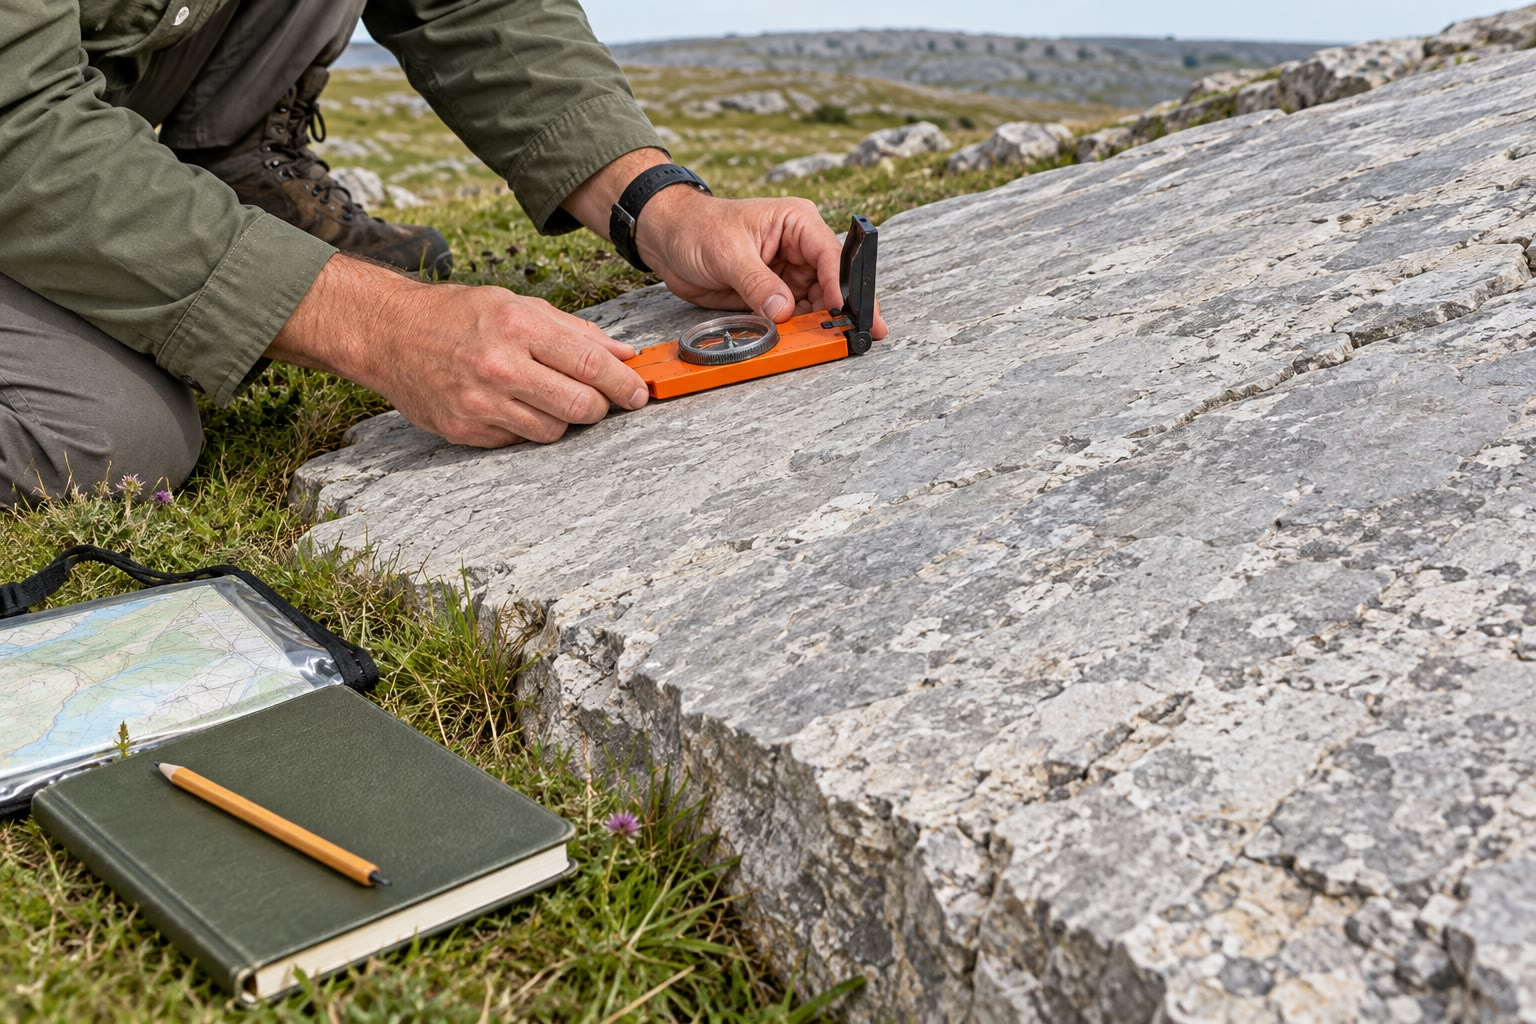
\includegraphics[width=0.6\linewidth]{images/book3/ai/b1-compass-clinometer.jpg}
\end{center}
\end{inthefield}

\begin{history}[أول خريطة جيولوجية لبلد]
% ledger: gsl:smith-1815, commons:smith-1815
عمل المساح ويليام سميث، الذي حفر القنوات وصرف الأراضي في إنجلترا، فلاحظ أن كل طبقة صخرية تحمل أحافيرها الخاصة، بترتيب واحد في كل مكان. فاستعمل الأحافير ليعرف الطبقات، وتتبّعها عبر البلد أكثر من خمس عشرة سنة. وخريطته، \emph{A Delineation of the Strata of England and Wales, with part of Scotland}، المؤرخة في 1 أغسطس 1815، تُعدّ أول \omterm{def:b1:geological-maps:geological-map}{خريطة جيولوجية} لبلد كامل.
\begin{center}
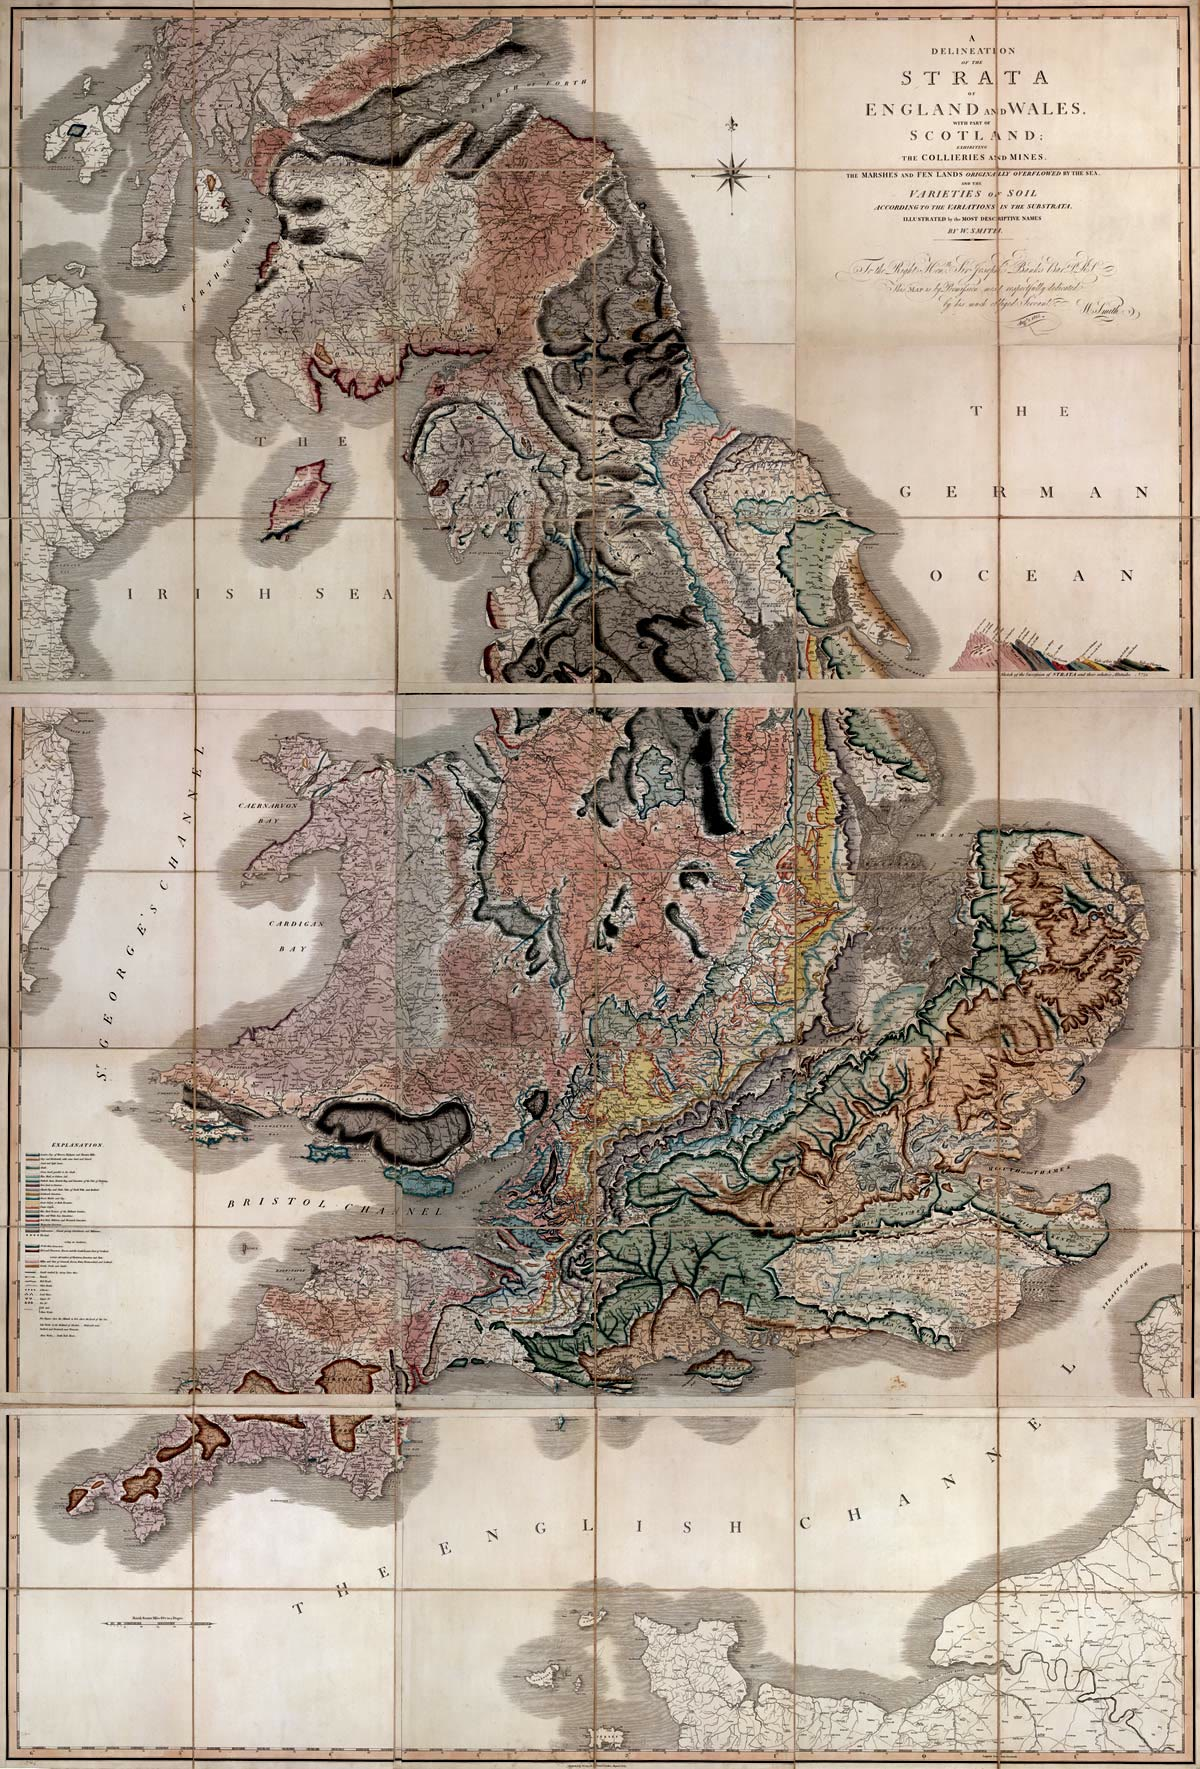
\includegraphics[width=0.36\linewidth]{images/book3/b1-smith-1815-map.jpg}

{\small خريطة ويليام سميث لعام 1815 (في الملك العام).}
\end{center}
\end{history}

\section{التمارين}

\begin{exercise}[$\star$]\label{exo:b1:geological-maps:1}
عرّف \omterm{def:b1:geological-maps:attitude}{الامتداد} \omterm{def:b1:geological-maps:attitude}{والانحدار} \omterm{def:b1:geological-maps:attitude}{واتجاه الانحدار} لمستوٍ. لطبقة وضعيتها $135/40$: أعطِ امتدادها وفق قاعدة اليد اليمنى، وارسم رمزها على الخريطة.
\end{exercise}

\begin{exercise}[$\star$]\label{exo:b1:geological-maps:2}
اكتب معادلة المستوي الذي وضعيته $090/30$ ويمرّ بالنقطة $(0, 0, 500)$، والإحداثيات بالمتر. على أيّ ارتفاع يكون عند $(1000, 0)$ وعند $(0, 1000)$؟
\end{exercise}

\begin{exercise}[$\star$]\label{exo:b1:geological-maps:3}
على خريطة، يتبع أثر تماسٍّ خطَّ الكنتور \qty{350}{m} بدقة، على امتداد عدة كيلومترات من التلال والأودية. ماذا يمكنك أن تقول عن هذا \omterm{def:b1:geological-maps:geological-map}{التماس}؟ وماذا لو كان أثره خطًّا مستقيمًا عبر التلال والأودية؟
\end{exercise}

\begin{exercise}[$\star$]\label{exo:b1:geological-maps:4}
على خريطة تلال فاردن، أيّ وحدة تنكشف في لبّ \omterm{def:b1:geological-maps:fold}{الطية المحدبة} على طول النهر، وأيّ وحدة تشغل لبّ \omterm{def:b1:geological-maps:fold}{الطية المقعرة}؟ علّل ذلك بمبدأ التراكب.
\end{exercise}

\begin{exercise}[$\star\star$]\label{exo:b1:geological-maps:5}
يُلاقى تماسٌّ عند الارتفاعات $\qty{300}{m}$ عند $(0, 0)$، و$\qty{300}{m}$ عند $(1000, 0)$، و$\qty{200}{m}$ عند $(0, 500)$ (بالأمتار، و$x$ نحو الشرق، و$y$ نحو الشمال). أوجد امتداده واتجاه انحداره وانحداره، أولًا بالاستدلال على الكنتورات البنيوية، ثم باستعمال \cref{thm:b1:geological-maps:three-point}.
\end{exercise}

\begin{exercise}[$\star\star$]\label{exo:b1:geological-maps:6}
ينحدر قاع وادٍ نحو الشمال بمقدار \qty{30}{m} لكل كيلومتر. في أيّ اتجاه يشير حرف V \omterm{def:b1:geological-maps:geological-map}{لانكشاف} \omterm{def:b1:geological-maps:geological-map}{تماس} إن كان \omterm{def:b1:geological-maps:geological-map}{التماس} (أ) أفقيًا؛ (ب) ينحدر \ang{20} نحو الجنوب؛ (ج) ينحدر \ang{1} نحو الشمال؛ (د) ينحدر \ang{20} نحو الشمال؟ علّل باستعمال \cref{thm:b1:geological-maps:v-rule}.
\end{exercise}

\begin{exercise}[$\star\star$]\label{exo:b1:geological-maps:7}
في وضع قاعدة V، يميل \omterm{def:b1:geological-maps:geological-map}{تماس} نحو المصب بمقدار $a = 0.364$ (\ang{20})، وينحدر قاع الوادي بمقدار $s = 0.03$. تقع نقطة على جانب الوادي أعلى من القاع بمقدار \qty{80}{m}. على أيّ بُعد أعلى المنبع من رأس الحرف يقع الأثر عند تلك النقطة؟
\end{exercise}

\begin{exercise}[$\star\star$]\label{exo:b1:geological-maps:8}
تُغلق \omterm{def:b1:geological-maps:geological-map}{انكشافات} \omterm{def:b1:geological-maps:fold}{طية} فاردن المحدبة حول الطرف الشمالي للبّها. في أيّ اتجاه يغوص \omterm{def:b1:geological-maps:fold}{محور الطية}؟ وهل تُغلق \omterm{def:b1:geological-maps:geological-map}{انكشافات} \omterm{def:b1:geological-maps:fold}{الطية المقعرة} نحو الشمال أم نحو الجنوب؟
\end{exercise}

\begin{exercise}[$\star\star$]\label{exo:b1:geological-maps:9}
على \omterm{def:b1:geological-maps:geological-map}{الخريطة الجيولوجية}، على طول الصدع: أيّ جانب يُظهر وحدات أحدث على السطح؟ وأيّ كتلة هبطت؟ تحقّق بالرمز على الخريطة.
\end{exercise}

\begin{exercise}[$\star\star\star$]\label{exo:b1:geological-maps:10}
بيّن أن مستويين وضعيتهما $(\alpha_1, \delta_1)$ و$(\alpha_2, \delta_2)$ يتقاطعان على خط موازٍ للمتجهة $\vec n_1 \times \vec n_2$، حيث $\vec n_i = (\tan\delta_i\sin\alpha_i,
\tan\delta_i\cos\alpha_i, 1)$. طبّق ذلك على المستويين $090/30$ و$270/30$: ما هذا الخط، وأيّ نوع من \omterm{def:b1:geological-maps:fold}{الطيات} يشكّله المستويان؟
\end{exercise}

\begin{exercise}[$\star\star\star$]\label{exo:b1:geological-maps:11}
يمتد سدّ شاقولي باتجاه \ang{045} ويُرى انكشافه عند نقطة الأصل، على قاع وادٍ ارتفاعه \qty{0}{m}. أين يمكن أن يقع أثره على تلّة ارتفاعها \qty{300}{m}؟ سدّ ثانٍ له \omterm{def:b1:geological-maps:attitude}{الامتداد} نفسه، ينحدر \ang{60} نحو الجنوب الشرقي، ويُرى انكشافه أيضًا عند نقطة الأصل. على أيّ بُعد من نقطة الأصل، وفي أيّ اتجاه، يقع أثره على أرض ارتفاعها \qty{300}{m}، مقيسًا عموديًا على \omterm{def:b1:geological-maps:attitude}{الامتداد}؟
\end{exercise}

\begin{exercise}[$\star\star\star$]\label{exo:b1:geological-maps:12}
في نموذج ارتفاع رقمي بشبكة \qty{100}{m}، ترتفع الأرض عند $(x, y)$ وعند $(x + 100, y)$ إلى 420 و\qty{405}{m}، وعند $(x, y + 100)$ إلى \qty{412}{m}. باعتبار الأرض في تلك الخلية مستوية، احسب ميلها (بالدرجات) \omterm{def:b1:spherical-astronomy:horizontal}{والسمت} الذي تواجهه (اتجاه الهبوط).
\end{exercise}

\section{مسألة: حلّ تلال فاردن}

\begin{problem}[{مسألة نهاية الأسبوع --- من الآبار الاستكشافية والخريطة إلى محور الطية والصدع وتاريخ المنطقة}]
\label{pb:b1:geological-maps:1}
% all data computed in figdata/bachelor-1/varden_maps.py from the region's
% model (figdata/shared/region.py); invented region: exercise data, no ledger
تحفر شركة مياه آبارًا في تلال فاردن، وتسجّل المواضع التي تلاقي فيها الآبار قاعدة الحجر الجيري؛ ويحدّد جيولوجيوها أيضًا موضع الصدع حيث يعبر الأرض. والإحداثيات بالأمتار شرقًا وشمالًا من الركن الجنوبي الغربي للخريطة؛ والارتفاعات بالأمتار فوق مستوى البحر. يستعمل الجزء الأول \omterm{def:b1:geological-maps:geological-map}{الخريطة الجيولوجية} الملوّنة في \cref{sec:b1:geological-maps:cut}.

\medskip
\noindent\textbf{الجزء الأول --- قراءة الخريطة.}
\begin{enumerate}
  \item أحصِ وحدات المنطقة من الأقدم إلى الأحدث.
  \item أيّ الوحدات يقطعها النهر، من الغرب إلى الشرق؟
  \item أيّ وحدة تشغل لبّ \omterm{def:b1:geological-maps:fold}{الطية} قرب $x = \qty{3.5}{km}$؟ وأيّ نوع من \omterm{def:b1:geological-maps:fold}{الطيات} هي؟
  \item أيّ وحدة تشغل لبّ \omterm{def:b1:geological-maps:fold}{الطية} قرب $x = \qty{7.5}{km}$؟ وأيّ نوع من \omterm{def:b1:geological-maps:fold}{الطيات} هي؟
  \item لماذا لا يظهر الشيست والغرانيت إلا قرب النهر، في لبّ \omterm{def:b1:geological-maps:fold}{الطية} الأولى؟
  \item أيّ نوع من التماسّ يفصل الحجر الرملي عن الغرانيت؟ علّل من الخريطة.
\end{enumerate}

\medskip
أما الآبار (العمق $d$ إلى قاعدة الحجر الجيري، والارتفاع الأرضي $z_g$) والنقاط الثلاث F1–F3 حيث يعبر الصدع قمة الصخر الأساسي (تقع F2 في الوادي تحت الطمي الرقيق الذي لا يقطعه الصدع): 

\begin{omfigure}
\begin{minipage}[c]{0.42\linewidth}
\centering\small
\begin{tabular}{lrrrr}
\hline
 & شرق & شمال & $z_g$ & $d$ \\
\hline
E1 & 4000 & 6000 & 435 & 261 \\
E2 & 4600 & 7200 & 432 & 428 \\
E3 & 5100 & 6400 & 512 & 586 \\
W1 & 1500 & 6000 & 524 & 669 \\
W2 & 2200 & 7200 & 421 & 459 \\
W3 & 2600 & 5400 & 319 & 209 \\
\hline
 & شرق & شمال & $z_g$ & \\
\hline
F1 & 4197 & 1000 & 405 & \\
F2 & 5824 & 3500 & 129 & \\
F3 & 7321 & 6500 & 482 & \\
\hline
\end{tabular}
\end{minipage}\hfill
\begin{minipage}[c]{0.56\linewidth}
\centering
\begin{tikzpicture}
\begin{axis}[axis equal image, xmin=0, xmax=10, ymin=0, ymax=8, width=\linewidth,
  tick label style={font=\scriptsize}, xlabel={\foreignlanguage{arabic}{الشرق \babelsublr{(\unit{km})}}}, ylabel={\foreignlanguage{arabic}{الشمال \babelsublr{(\unit{km})}}},
  label style={font=\footnotesize}]
\addplot[fill=black!8, draw=black!50, line width=0.3pt, even odd rule] table {figdata/out/shared-region-unit-schist.dat};
\addplot[fill=black!8, draw=black!50, line width=0.3pt, even odd rule] table {figdata/out/shared-region-unit-granite.dat};
\addplot[fill=icsTriassic!20, draw=black!50, line width=0.3pt, even odd rule] table {figdata/out/shared-region-unit-sandstone.dat};
\addplot[fill=icsJurassic!25, draw=black!50, line width=0.3pt, even odd rule] table {figdata/out/shared-region-unit-limestone.dat};
\addplot[fill=icsJurassic!8, draw=black!50, line width=0.3pt, even odd rule] table {figdata/out/shared-region-unit-shale.dat};
\addplot[fill=icsCretaceous!20, draw=black!50, line width=0.3pt, even odd rule] table {figdata/out/shared-region-unit-chalk.dat};
\addplot[fault] table {figdata/out/shared-region-fault.dat};
\addplot[fill=omLithAlluv, draw=black!50, line width=0.3pt, even odd rule] table {figdata/out/shared-region-unit-alluvium.dat};
\addplot[river] table {figdata/out/shared-region-river.dat};
\addplot[only marks, mark=*, mark size=1.6pt] table[x=x_km, y=y_km] {figdata/out/bachelor-1-varden_maps-boreholes.dat};
\addplot[only marks, mark=square*, mark size=1.5pt, omThm] table[x=x_km, y=y_km] {figdata/out/bachelor-1-varden_maps-fault.dat};
\begin{scope}[every node/.style={font=\scriptsize\bfseries, inner sep=1.5pt, fill=white, fill opacity=0.8, text opacity=1}]
  \node[above right] at (axis cs:4,6) {E1};
  \node[above] at (axis cs:4.6,7.2) {E2};
  \node[right] at (axis cs:5.1,6.4) {E3};
  \node[above left] at (axis cs:1.5,6) {W1};
  \node[above] at (axis cs:2.2,7.2) {W2};
  \node[left] at (axis cs:2.6,5.4) {W3};
  \node[left, text=omThm] at (axis cs:4.197,1) {F1};
  \node[left, text=omThm] at (axis cs:5.824,3.5) {F2};
  \node[left, text=omThm] at (axis cs:7.321,6.5) {F3};
\end{scope}
\end{axis}
\end{tikzpicture}
\end{minipage}
\end{omfigure}

\medskip
\noindent\textbf{الجزء الثاني --- الجناح الشرقي.}
\begin{enumerate}[resume]
  \item احسب ارتفاع قاعدة الحجر الجيري في E1 وE2 وE3.
  \item اكتب المتجهتين $\overrightarrow{E_1E_2}$ و$\overrightarrow{E_1E_3}$.
  \item احسب جداءهما المتجهي، ووجّهه نحو الأعلى.
  \item استنتج انحدار قاعدة الحجر الجيري على الجناح الشرقي.
  \item استنتج اتجاه انحدارها، ثم امتدادها وفق قاعدة اليد اليمنى.
  \item هل تتفق النتيجة مع رمز \omterm{def:b1:geological-maps:attitude}{الامتداد} \omterm{def:b1:geological-maps:attitude}{والانحدار} للجناح الشرقي على الخريطة؟
\end{enumerate}

\medskip
\noindent\textbf{الجزء الثالث --- \omterm{def:b1:geological-maps:fold}{الطية}.}
\begin{enumerate}[resume]
  \item احسب ارتفاعات قاعدة الحجر الجيري في W1 وW2 وW3.
  \item احسب ناظمًا نحو الأعلى $\vec n_W$ لقاعدة الحجر الجيري على الجناح الغربي.
  \item استنتج \omterm{def:b1:geological-maps:attitude}{وضعية} الجناح الغربي.
  \item احسب اتجاه تقاطع الجناحين، أي \omterm{def:b1:geological-maps:fold}{محور الطية}، بوصفه $\vec n_E \times \vec n_W$ (مع $\vec n_E$ من السؤال 9).
  \item أعطِ الاتجاه (سمت الإسقاط الأفقي للمحور، مأخوذًا نحو الأسفل) والغوص (زاوية المحور تحت الأفق) \omterm{def:b1:geological-maps:fold}{لمحور الطية}.
  \item تقع قاعدة الحجر الرملي على المحور عند \qty{230}{m} حيث يعبره النهر، قرب $y = \qty{4}{km}$. بكم تنخفض عليه على بُعد \qty{8}{km} أبعد نحو الشمال؟ وهل يتّسق ذلك مع السؤال 3 من الجزء الأول ومع إغلاق \omterm{def:b1:geological-maps:geological-map}{الانكشافات}؟
\end{enumerate}

\medskip
\noindent\textbf{الجزء الرابع --- الصدع والتاريخ.}
\begin{enumerate}[resume]
  \item انطلاقًا من F1 وF2 وF3، احسب \omterm{def:b1:geological-maps:attitude}{وضعية} الصدع.
  \item على طول الصدع، الوحدات الظاهرة على السطح في الجانب الشرقي الجنوبي الشرقي أحدث من التي تقابلها. أيّ كتلة هبطت؟ هل الصدع عادي أم معكوس؟
  \item يمرّ الخط المستقيم من F1 إلى F3 على بُعد نحو \qty{200}{m} غرب F2. لماذا ينحني أثر الصدع نحو الشرق الجنوبي الشرقي عندما يعبر وادي النهر، عند F2؟
  \item رتّبها زمنيًا: الطيّ؛ ترسيب الطباشير؛ الصدع؛ اقتحام الغرانيت؛ التعرية قبل الحجر الرملي؛ ترسيب الطمي.
  \item الطباشير عمرها 90 مليون سنة وهي مطوية؛ والطمي تكوّن في آخر 2.58 مليون سنة ولم يصبه الصدع. بين أيّ عمرين وقعت الطيّ والصدع؟
  \item لبلوغ الصدع على عمق \qty{1000}{m} تحت مستوى البحر أسفل F1، على أيّ بُعد من F1، وفي أيّ اتجاه، يجب أن تُحفر بئر رأسية؟
\end{enumerate}
\end{problem}
